\chapter{Électronique des Resistive Plate Chamber}
\renewcommand\chapterillustration{ELE/ele}
\ThisULCornerWallPaper{1}{\chapterillustration}
\minitoc

\lettrine[lines=4, slope=-0.5em]{C}{e} chapitre présente le développement d'un nouveau type de PCB avec lecture des deux côté des strips. Cette configuration permet, grâce au temps de propagation du signal de connaitre la position du hit le long du strip touché. Ce chapitre présente également les premiers résultats obtenus lors de tests en faisceaux au SPS en mai 2017.

\section{Principe de fonctionnement}

Chaque chambres actuels de CMS ont un PCB segmentés en trois zones selon $\eta$ appelées "$\eta$ segments", chaque $\eta$ segments contenant \num{32} strips. Lors du passage d'un muon, la position de celui-ci selon $\eta$ n'est connu qu'avec une résolution correspondant à la longueur du strip touché.

Afin de résoudre ce problème et d'éviter la segmentation en $\eta$ du PCB, un type de PCB permettant la lecture des deux côté des strip a été proposé (cf.fig~\ref{PCB1}).

\begin{figure}[ht!]
	\centering
	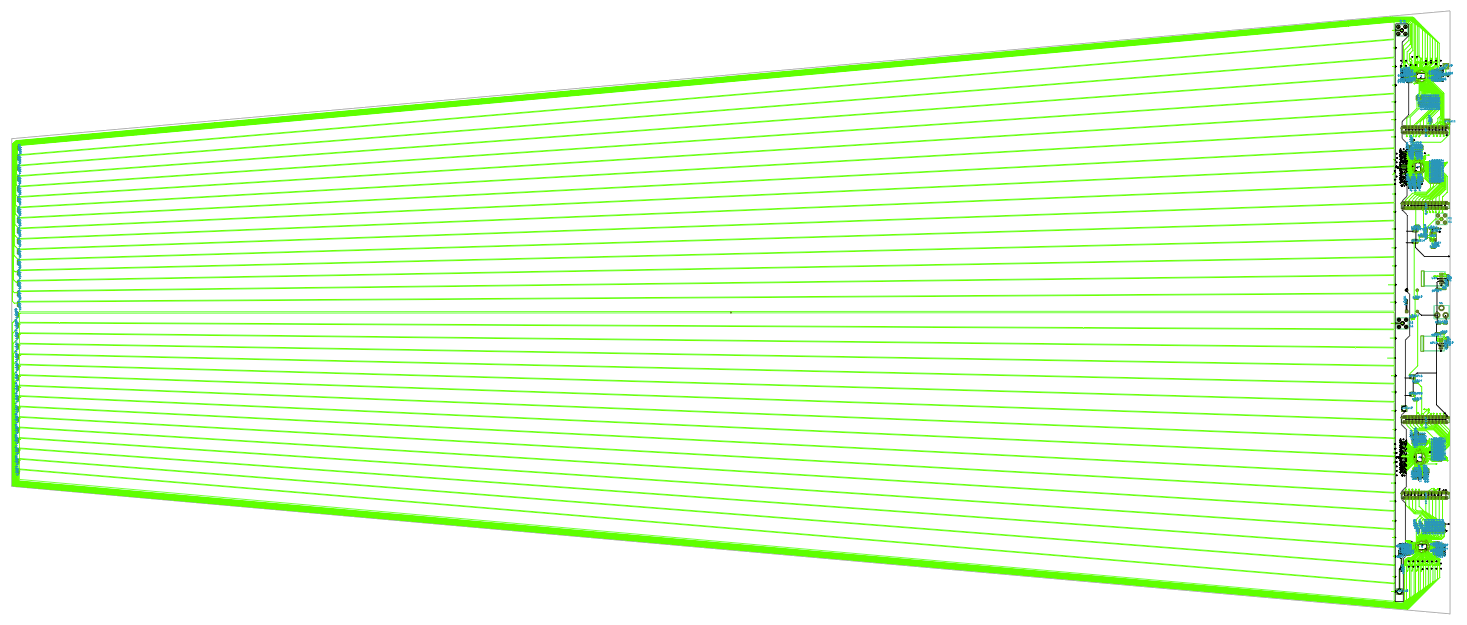
\includegraphics[width=0.90\textwidth]{ELE/PCB1.png}
	\captionof{figure}{Schèma du PCB permettant la lecture des deux côté des strips.}
	\label{PCB1}
\end{figure}

Les strips font toute la longeur de la chambre, chaque bouts du strips est relié à une voie d'électronique. Le retour du strips est effectué sur les côté du PCB, dans une zone protéger par un blindage relié à la masse afin qu'il ne soit pas affecter par le passage des particules.

Ce type de configuration permet de connaitre la position du hits le long du strips. En effet en posant $L$ la longueur de la ligne (strip et retour), $Y$ la position du hits le long du strips, $t_1$ et $t_2$ le temps de propagation du signal pour rejoindre l'un est l'autre côté de la ligne et $v$ la vitesse de propagation du signal :
\begin{equation}
Y=\frac{L}{2}-\frac{v(t_2-t_1)}{2}
\end{equation} 

La résolution temporelle du signal peut également être calculé :
\begin{equation}
\sigma_{t}=(t_1+t_2)-\frac{L}{v}
\end{equation}

\subsection{Le Prototype}
Afin d'étudier la faisabilité, un PCB de \SI{50}{\centi\meter} de long a été créé (cf.fig~\ref{PCB2}). Il est composé de \num{32} strips espacé de \SI{4}{\milli\meter}. Ces strips sont lus de chaque côté grâce à \num{2} ASIC appelé PETIROC2 \cite{Monzo:2017quz} de \num{32} entrées, développé par le groupe OMEGA. Ces ASIC sont utilisés pour mettre en forme les signaux. Deux TDC de \num{24} voies chacun et de résolution temporelle \SI{25}{\nano\second}, développés par nos collègue de Tsinghua sont utilisé afin de mesurer le temps d'arrivé des signaux envoyé par les PETIROC2.

\begin{figure}[ht!]
	\centering
	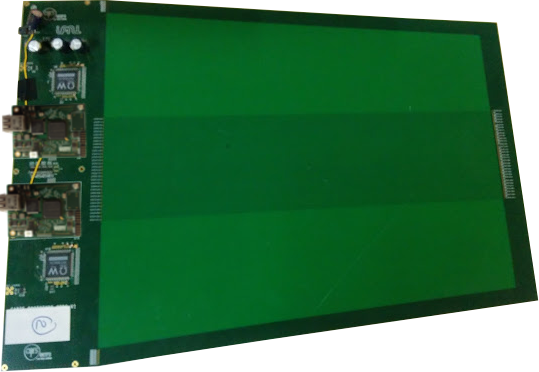
\includegraphics[width=0.50\textwidth]{ELE/PCB2.png}
	\captionof{figure}{Le PCB avec lecture des strips des deux côtés.}
	\label{PCB2}
\end{figure}

\subsubsection{L'ASIC PETIROC2}
\begin{wrapfigure}[8]{R}{0.40\textwidth}
	\vspace*{-1cm}
	\centering
	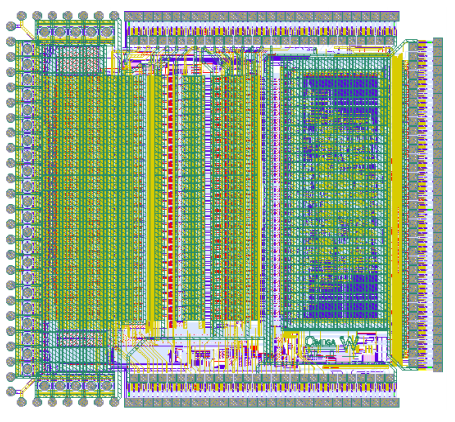
\includegraphics[width=0.37\textwidth]{ELE/PETIROC.png}
	\caption{Schéma électronique du PETIROC2.}
	\label{PETIROC2}
\end{wrapfigure}
Le PETIROC2 (cf.fig~\ref{PETIROC2}) possède une gigue\footnote{La gigue ou \textit{jitter} en anglais, provient des fluctuations statistiques et du bruit de l'électronique. À cause de ces fluctuations, deux signaux identiques ne vont pas passer le seuil de déclenchement au même point, donnant ainsi une variation temporelle du point de déclenchement qui dépend de l'amplitude des fluctuations.} faible ($<\SI{20}{\pico\second}$ pour une charge supérieur à \SI{160}{\femto\coulomb}). Le schéma simplifié du PETIROC2 est donné figure \ref{SchemePETIROC}. Cette ASIC dispose de \num{32} voies permettant de mesurer le temps de vol grâce à un TDC intégré et un ADC de 10bits ainsi que la charge sur 10bits. La gamme de réglage du seuil est compris entre \SI{160}{\femto\coulomb} et \SI{400}{\pico\coulomb} global aux \num{32} voies. Un ajustement voie par voie est possible grâce à un DAC de 6bits. 

\begin{figure}[ht!]
	\centering
	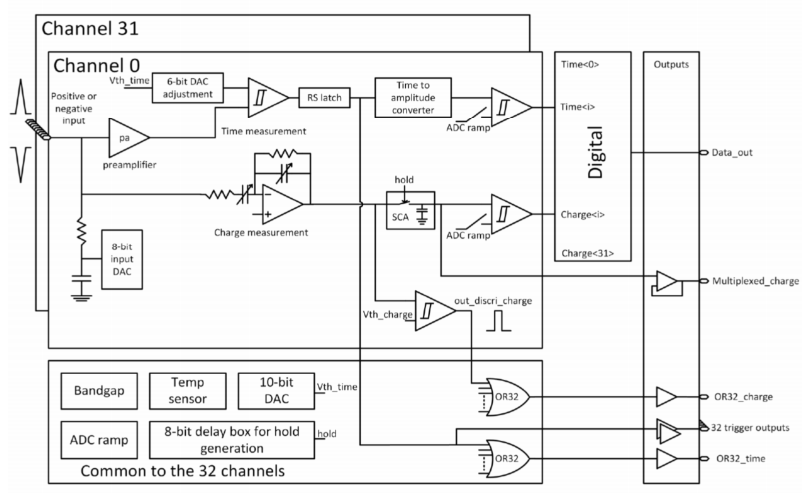
\includegraphics[width=0.90\textwidth]{ELE/Scheme.png}
	\captionof{figure}{schéma simplifié du PETIROC2.}
	\label{SchemePETIROC}
\end{figure}

\subsubsection{Le TDC}
\begin{wrapfigure}[8]{R}{0.40\textwidth}
	\vspace*{-1cm}
	\centering
	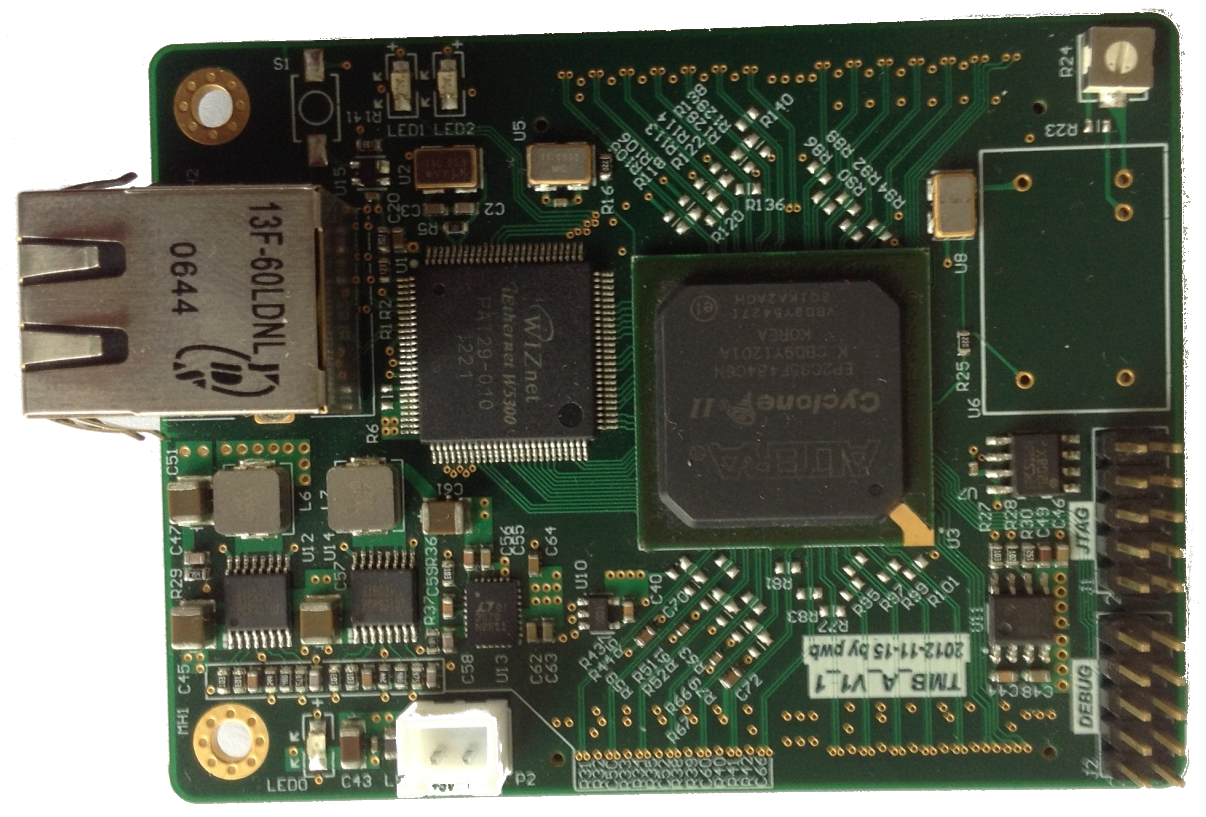
\includegraphics[width=0.37\textwidth]{ELE/TDC.png}
	\caption{Un TDC fournit par nos collègues de Tsinghua.}
	\label{tdc}
\end{wrapfigure}
Le TDC fournit par nos collègues chinois possède \num{24} voies et une résolution temporelle de \SI{25}{\pico\second}. Il est basé sur un FPGA de type Cyclone-II. Cette carte reçoit les données des PETIROC2 grêce à des connecteur à entrées différentielles. Les données sont envoyées grâce à un port Éthernet utilisant les protocoles TCP\footnote{Transmission Control Protocol.}/IP\footnote{Internet Protocol.}.